\documentclass[11pt]{article}

\usepackage[a4paper,margin=1in]{geometry}
\usepackage{setspace}
\usepackage{lineno}
\usepackage{graphicx}
\usepackage{float}
\usepackage{booktabs}
\usepackage{amsmath}
\usepackage{caption}
\usepackage{authblk}
\usepackage{natbib}
\usepackage[hidelinks]{hyperref}
\usepackage{url}
\usepackage{pdflscape}
\usepackage{longtable}

\graphicspath{{../figures/exploratory/}{../figures/fitted_curves/}{../figures/summary/}}

\setstretch{1.5}
\bibliographystyle{apalike}
\urlstyle{same}

\begin{document}

%========================
% Title page
%========================
\begin{titlepage}
    \centering
    \vspace*{2cm}

    {\LARGE \textbf{Logistic models more often outperform Gompertz models for empirical microbial growth curves}}\\[1.5cm]

    {\Large Ruixuan Han}\\[0.5cm]
    {\large Imperial College London}\\[1cm]

    {\large Word count: 1981}\\[2cm]

    \vfill
\end{titlepage}

%========================
% Abstract
%========================
\begin{abstract}
Population growth curves are central to ecology, microbiology, and food biology because they summarise how organisms respond to environmental conditions and resource limitation. However, empirical growth data often vary substantially in shape, making it unclear whether a single mathematical form adequately captures observed trajectories. Here I compared two common sigmoidal growth models, the logistic and Gompertz models, using a heterogeneous empirical dataset of microbial growth curves collected across multiple species, temperatures, media, and published studies.

I cleaned the course-provided Population Growth dataset, inferred individual growth curves from combinations of citation, species, temperature, medium, and replicate, and fitted both models separately to each curve using non-linear least squares. Models were compared using Akaike's Information Criterion (AIC), with Bayesian Information Criterion (BIC) and residual patterns used as secondary diagnostics.

After cleaning, the dataset contained 4262 observations across 297 growth curves, spanning 45 species, 17 temperature levels, and 18 media types. Model fitting was highly successful overall, with only one failed logistic fit. Logistic models provided the lowest AIC for 176 curves, whereas Gompertz models were best for 121 curves. Representative fits showed that both models described many monotonic sigmoidal trajectories well, but both performed poorly for curves that declined after reaching a peak.

Overall, the logistic model was the more robust general-purpose description of these microbial growth data, although the Gompertz model remained competitive for a substantial subset of curves. These results suggest that model choice matters for empirical growth analysis, and that broader candidate model sets may be needed when growth trajectories depart from simple asymptotic forms.
\end{abstract}

\newpage
\linenumbers

%========================
% Introduction
%========================
\section{Introduction}

Population growth is a foundational concept in biology because changes in abundance through time reflect the combined effects of physiology, resource availability, environmental conditions, and density dependence. In microbial systems, growth curves are especially important because they are used to describe spoilage dynamics, fermentation performance, laboratory culture behaviour, and environmental responses across taxa and conditions \citep{Zwietering1990}. A useful growth model should therefore provide both a good statistical fit and a biologically interpretable representation of observed dynamics.

Several mathematical models have been used to describe sigmoidal growth. The logistic equation is a classic density-dependent model in which growth slows as population size approaches an upper asymptote \citep{Verhulst1838}. The Gompertz model is another sigmoidal form that is often more asymmetric and has been widely used in microbial growth studies \citep{Gompertz1825,Zwietering1990}. Because these models differ in flexibility and shape, they can lead to different conclusions when fitted to empirical data. Model comparison is therefore not only a descriptive exercise, but also a way to evaluate alternative biological hypotheses about how growth unfolds through time \citep{JohnsonOmland2004}.

Here I ask which of two common sigmoidal growth models, logistic or Gompertz, better describes an empirical dataset of microbial population growth curves collected across many species and experimental conditions. Specifically, I ask: (1) how often each model provides the best fit across curves; (2) whether model preference varies across temperatures; and (3) what kinds of curve shapes are poorly captured by both models.

%========================
% Methods
%========================
\section{Methods}

\subsection{Data}

I used the Population Growth dataset supplied for the MQB mini project. The course page specifies that this dataset contains microbial growth observations with columns for time, biomass response, temperature, units, species, medium, replicate, and citation, and that individual growth curves must be inferred from combinations of metadata rather than from a pre-existing curve ID \citep{MQBMiniProject}. The response variable (\texttt{PopBio}) is recorded in multiple unit types, including OD\_595, CFU, dry weight, and population count, while time is recorded in hours \citep{MQBMiniProject}.

The cleaned dataset used here contained 4262 observations. Individual curves were defined by unique combinations of \texttt{Citation}, \texttt{Species}, \texttt{Temp}, \texttt{Medium}, and \texttt{Rep}, yielding 297 curves for model fitting.

\subsection{Data cleaning}

I first removed an extraneous index-like column and coerced the \texttt{Time}, \texttt{PopBio}, \texttt{Temp}, and \texttt{Rep} fields to numeric type where appropriate. Records with missing values in essential fields were removed. I retained only observations with non-negative time and strictly positive biomass, because both candidate models assume positive state variables and because log-based starting value estimation requires positive responses.

Growth curves were then sorted by time within each inferred curve ID. Curves containing fewer than five observations were excluded before fitting, because three-parameter non-linear models are unstable on extremely short series. This filtering reduced the dataset from approximately 305 inferred curves to 297 fitted curves.

\subsection{Candidate models}

I compared two three-parameter sigmoidal growth models.

The logistic model was fitted as:

\begin{equation}
N(t) = \frac{K}{1 + \left(\frac{K-N_0}{N_0}\right)e^{-rt}},
\end{equation}

where $N(t)$ is biomass at time $t$, $K$ is the asymptotic population size, $r$ is the intrinsic growth parameter, and $N_0$ is the initial population size.

The Gompertz model was fitted as:

\begin{equation}
N(t) = K \exp\left[-\exp\left(-r(t-t_0)\right)\right],
\end{equation}

where $K$ is the upper asymptote, $r$ is a growth-rate-related shape parameter, and $t_0$ controls the horizontal position of the inflection region.

These two models were chosen because both are standard in population and microbial growth analysis, but they differ in symmetry and flexibility \citep{Zwietering1990}.

\subsection{Model fitting and selection}

Each curve was fitted independently using non-linear least squares in Python. Initial values were estimated automatically from each curve using observed minima, maxima, median time, and a crude slope estimate from the log-transformed response.

For each fitted model I recorded parameter estimates, residual sum of squares (RSS), Akaike's Information Criterion (AIC), Bayesian Information Criterion (BIC), and convergence status. The primary model-selection criterion was AIC, because the two candidate models had equal parameter counts but potentially different fit quality \citep{JohnsonOmland2004}. Lower AIC indicates the better-supported model for a given curve. BIC was retained as a secondary comparison metric.

\subsection{Computing tools}

The final reproducible workflow combined Python, bash, Git, and \LaTeX. The workflow was implemented as separate Python scripts: \texttt{data\_prep.py} for data cleaning and curve-ID construction, \texttt{fit\_models.py} for non-linear model fitting and export of model metrics, and \texttt{analysis\_and\_plots.py} for model comparison, summary tables, and figure generation. A top-level script, \texttt{run\_MiniProject.py}, ran the workflow, while \texttt{compile\_report.py} compiled the final report.

Within Python, \texttt{pandas} was used for tabular data handling, \texttt{NumPy} for numerical operations, \texttt{SciPy} for non-linear optimisation, and \texttt{matplotlib} for plotting. Bash and shell commands were used to execute the workflow and compile the final \LaTeX{} report from the command line. Git was used for version control and project organisation. The report itself was written in \LaTeX{}, and references were managed with BibTeX. Although R was covered in the course and considered during project planning, it was not used in the final workflow because the analysis was intentionally kept within a single-language Python pipeline for clarity, consistency, and reproducibility.

%========================
% Results
%========================
\section{Results}

\subsection{Data overview}

After cleaning, the dataset contained 4262 observations across 297 microbial growth curves. These curves spanned 45 species, 17 temperature levels, and 18 growth media. Time was recorded in hours throughout the dataset, but biomass units varied among OD\_595, CFU, dry weight, and population count. Because of this unit heterogeneity, model comparison was performed within curves rather than by comparing parameter magnitudes across all curves.

Most growth curves contained relatively few observations, with a strong concentration between roughly 5 and 20 time points, although a small number of curves were much longer (Figure~\ref{fig:curvepoints}). Temperature representation was also uneven, with the largest number of curves occurring at 15$^\circ$C and substantial additional representation at 20, 25, and 35$^\circ$C (Figure~\ref{fig:temperaturecounts}). The dataset was taxonomically broad, although several species contributed disproportionately many curves (Figure~\ref{fig:speciescounts}).

\begin{figure}[H]
    \centering
    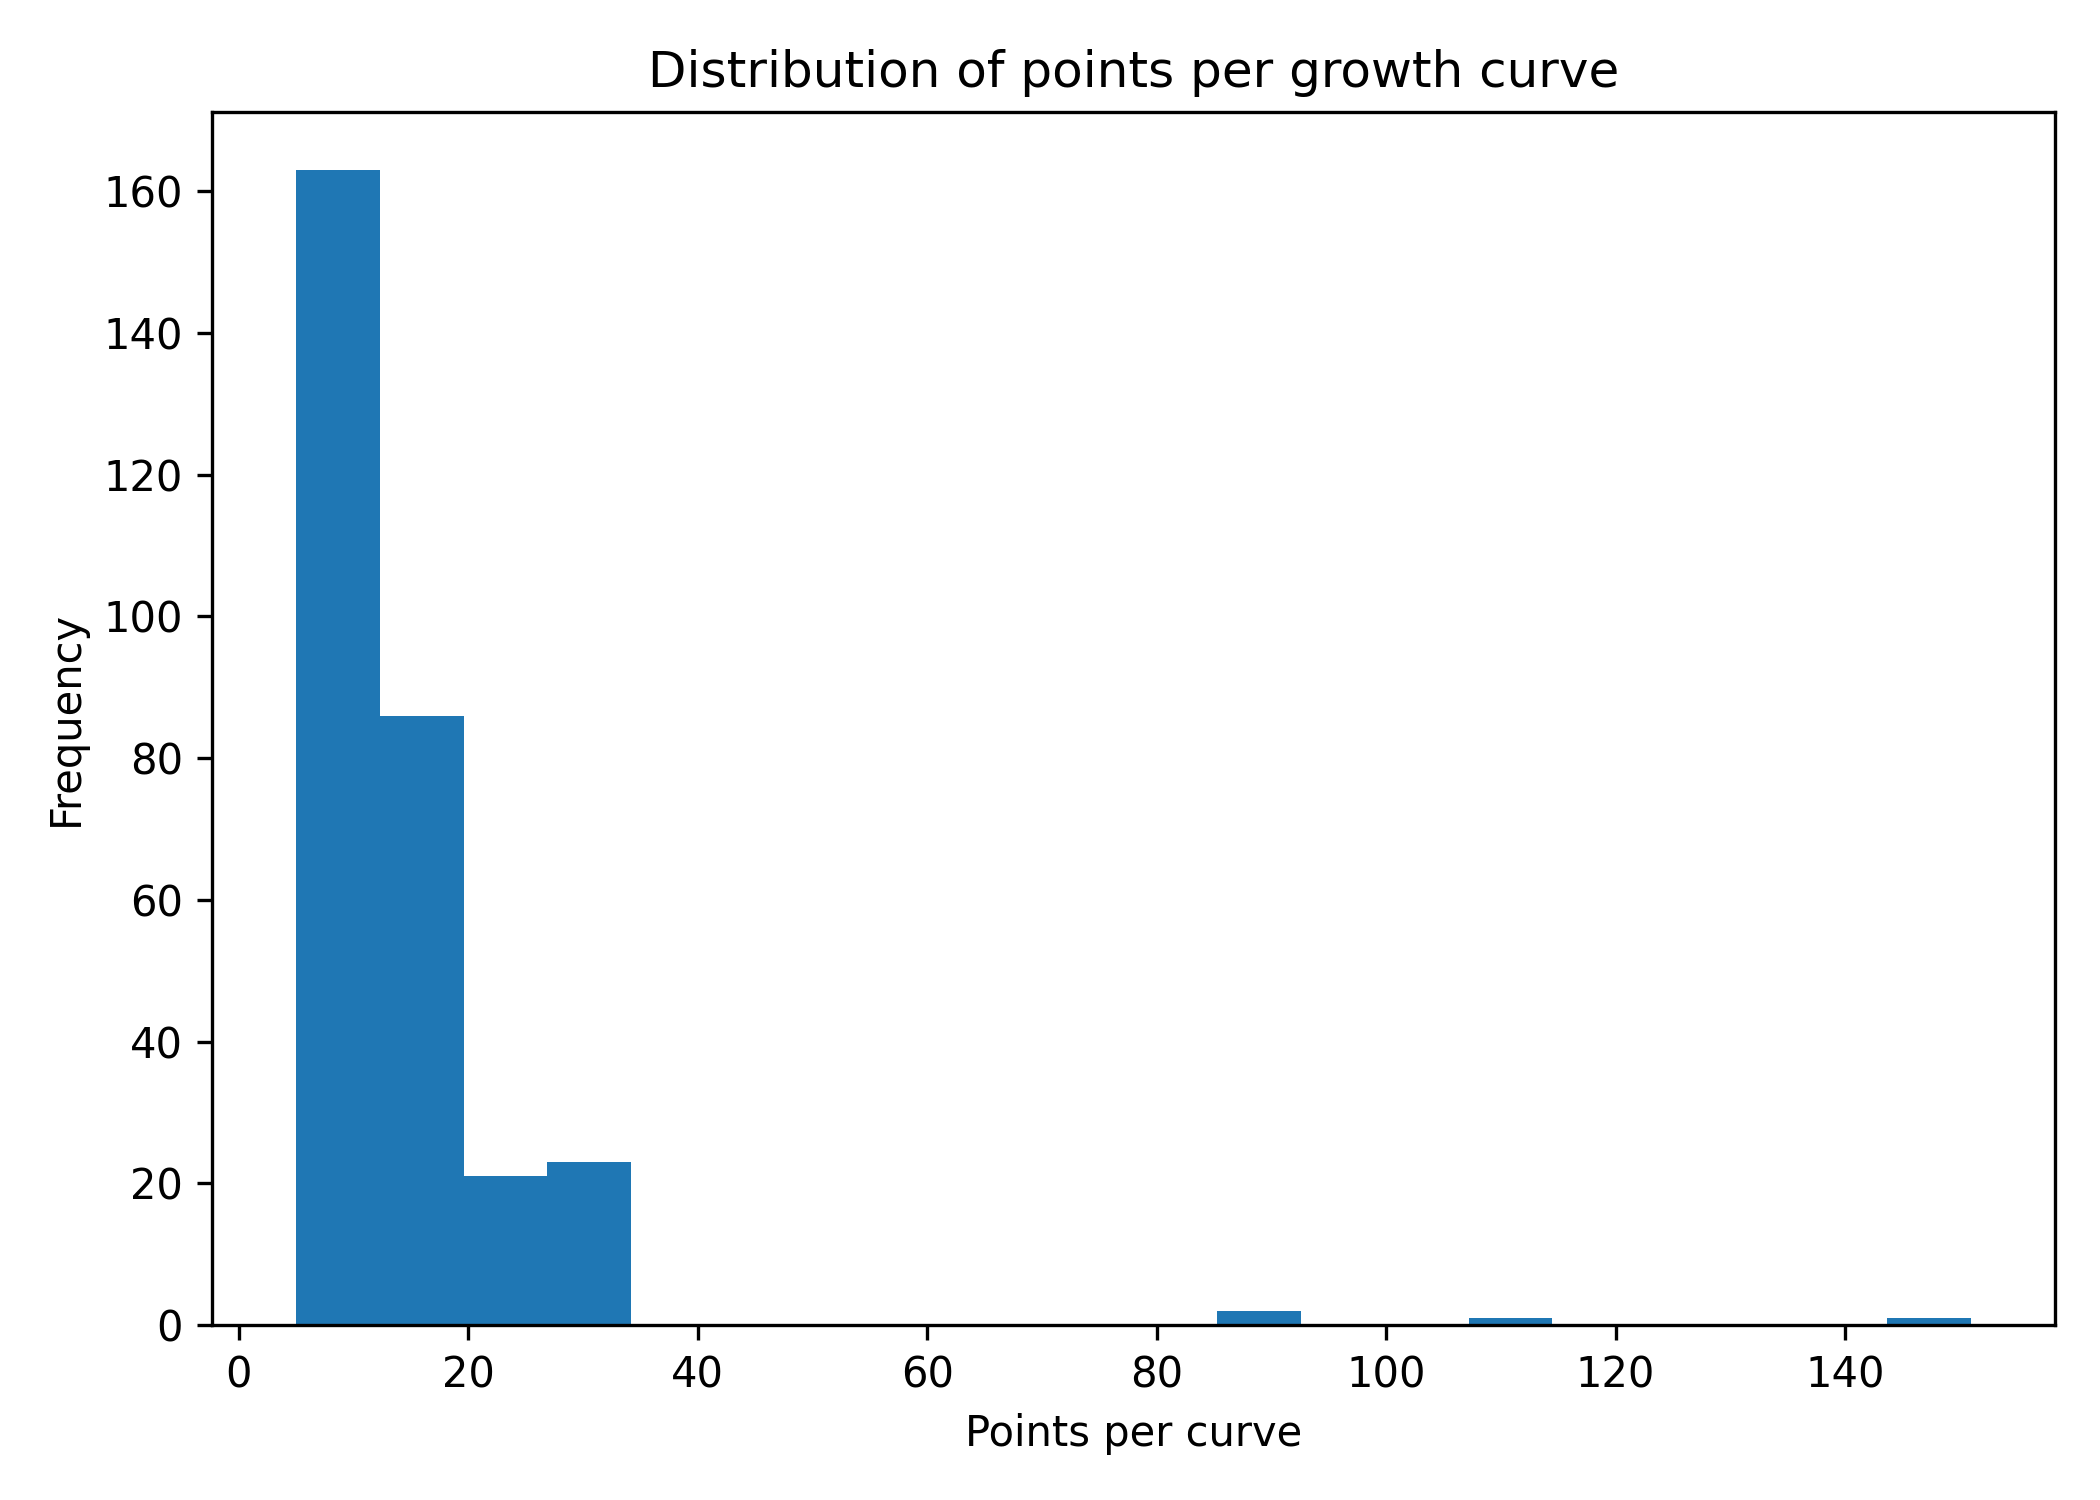
\includegraphics[width=0.75\textwidth]{curve_point_distribution.png}
    \caption{Distribution of observations per growth curve after cleaning. Most curves contained between 5 and 20 observations, with a small number of much longer time series. This justified excluding extremely short curves before fitting.}
    \label{fig:curvepoints}
\end{figure}

\begin{figure}[H]
    \centering
    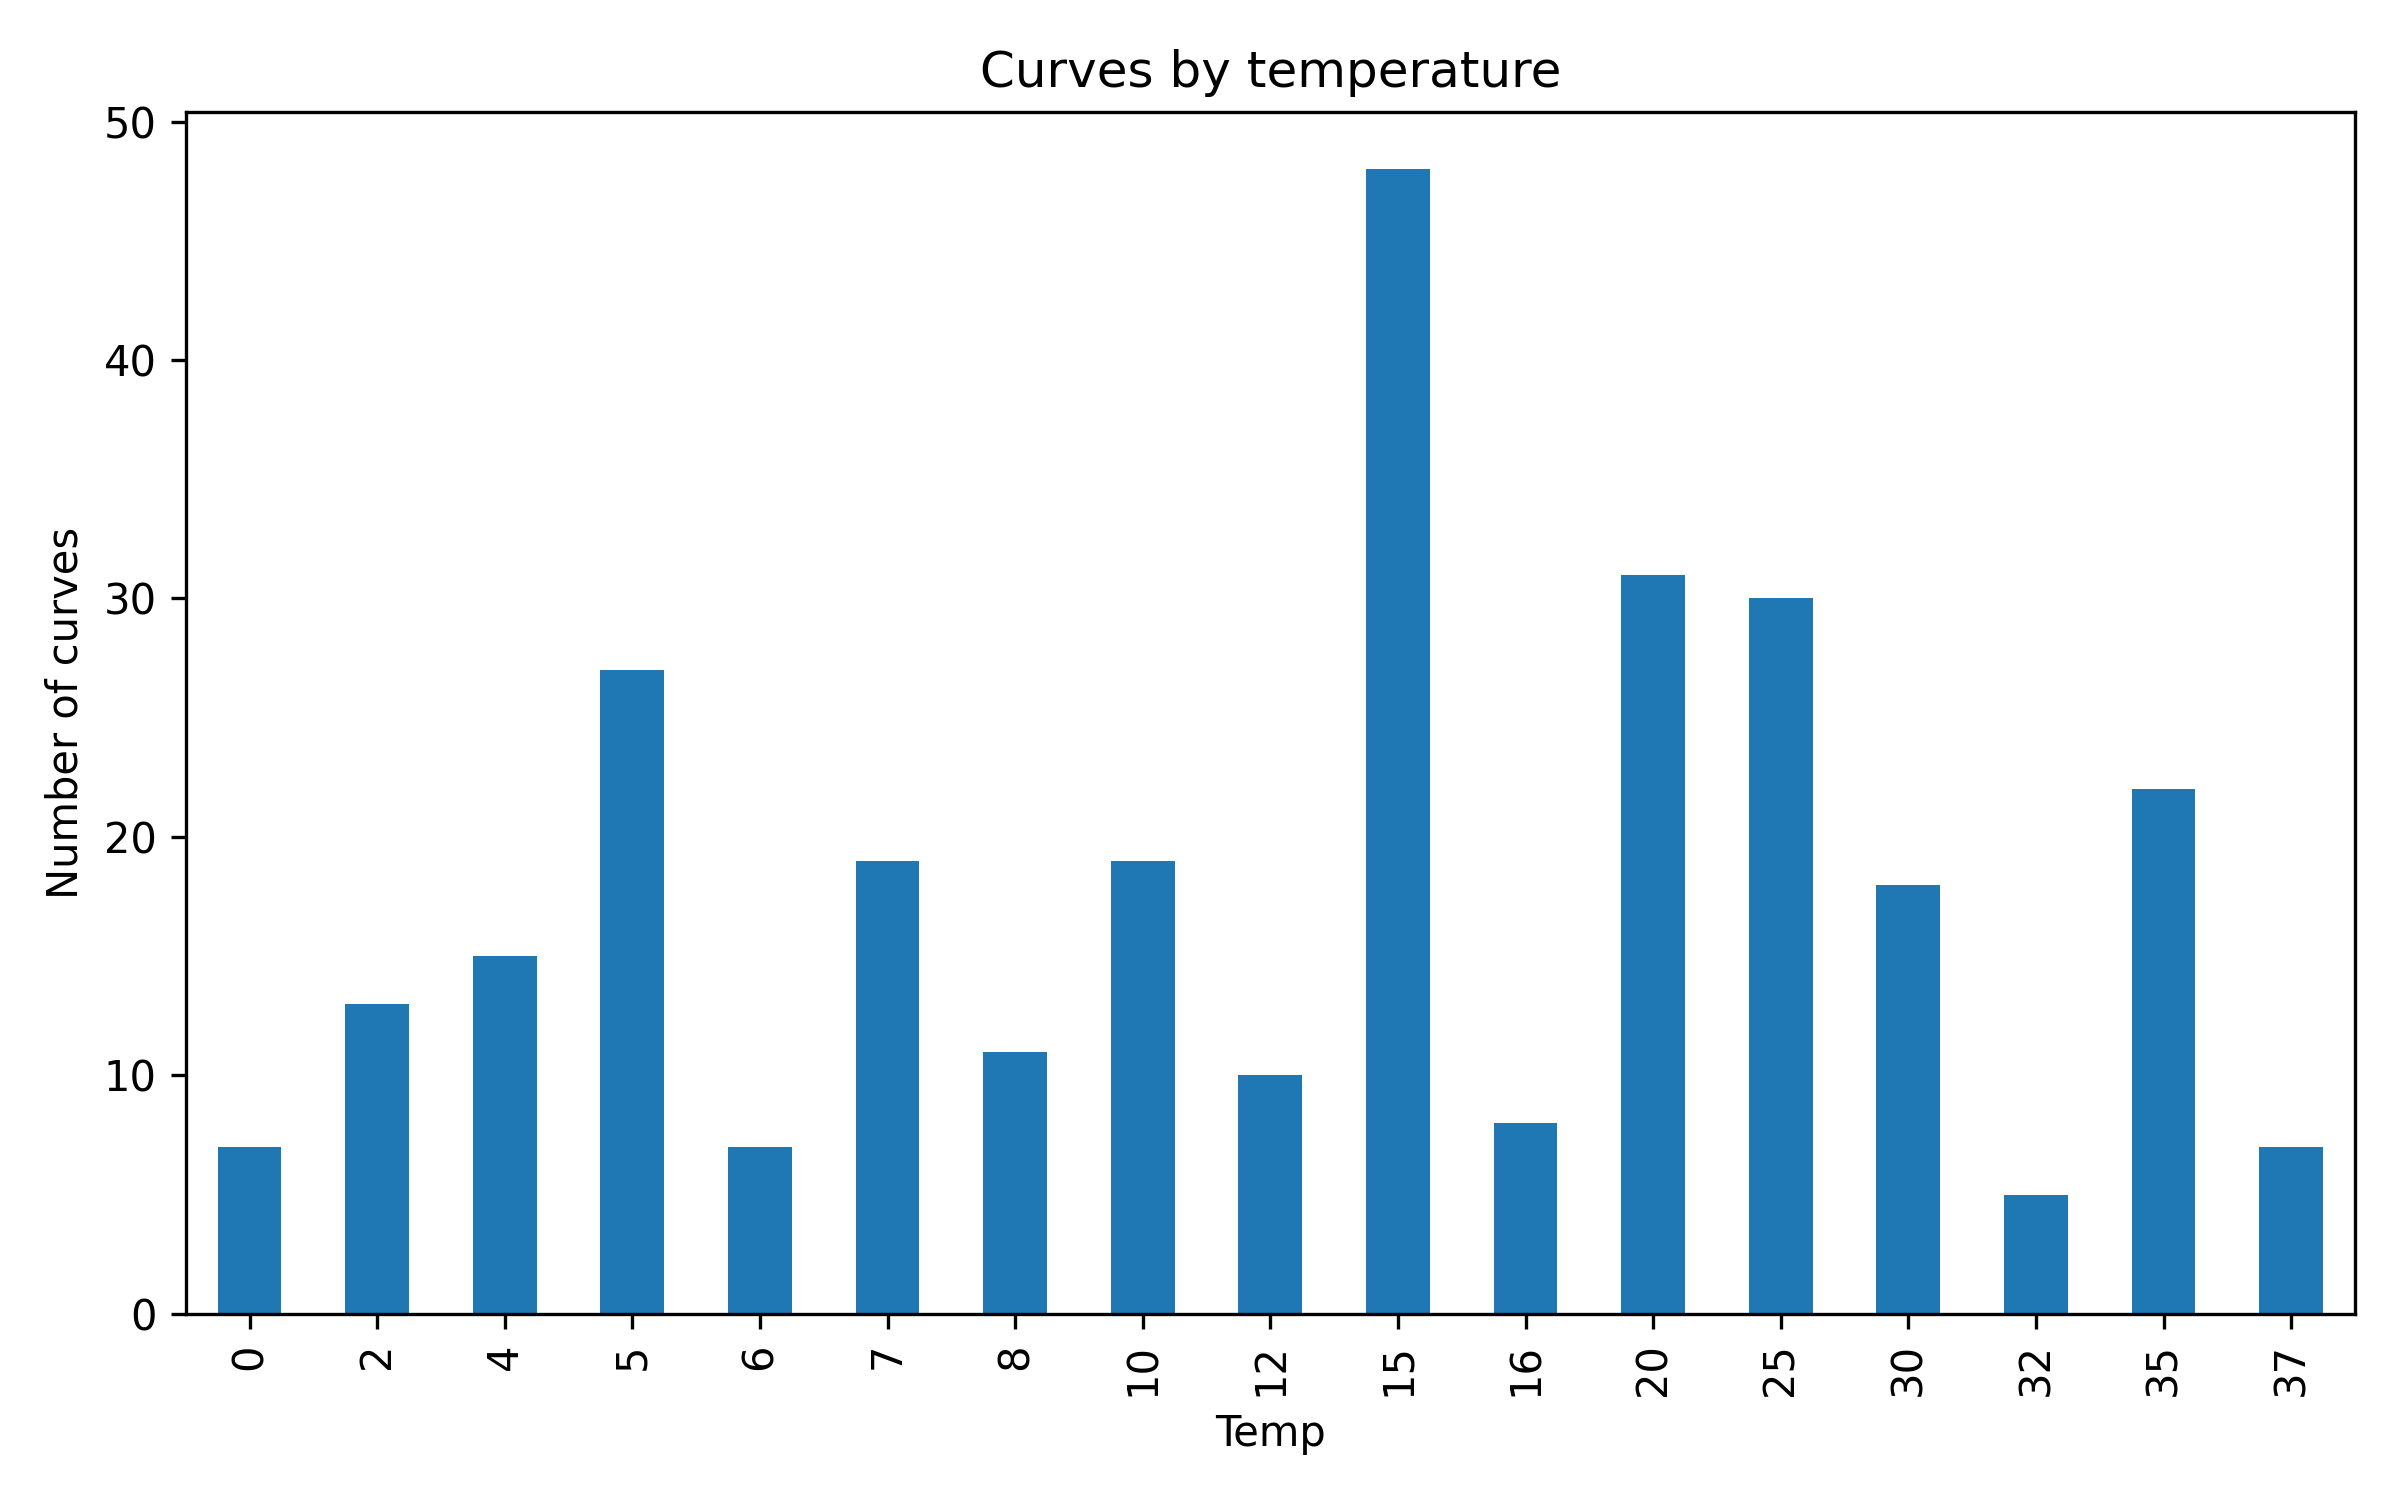
\includegraphics[width=0.8\textwidth]{temperature_curve_counts.png}
    \caption{Number of fitted curves at each temperature. Sampling effort was uneven across temperatures, which should be considered when interpreting temperature-specific model proportions.}
    \label{fig:temperaturecounts}
\end{figure}

\begin{figure}[H]
    \centering
    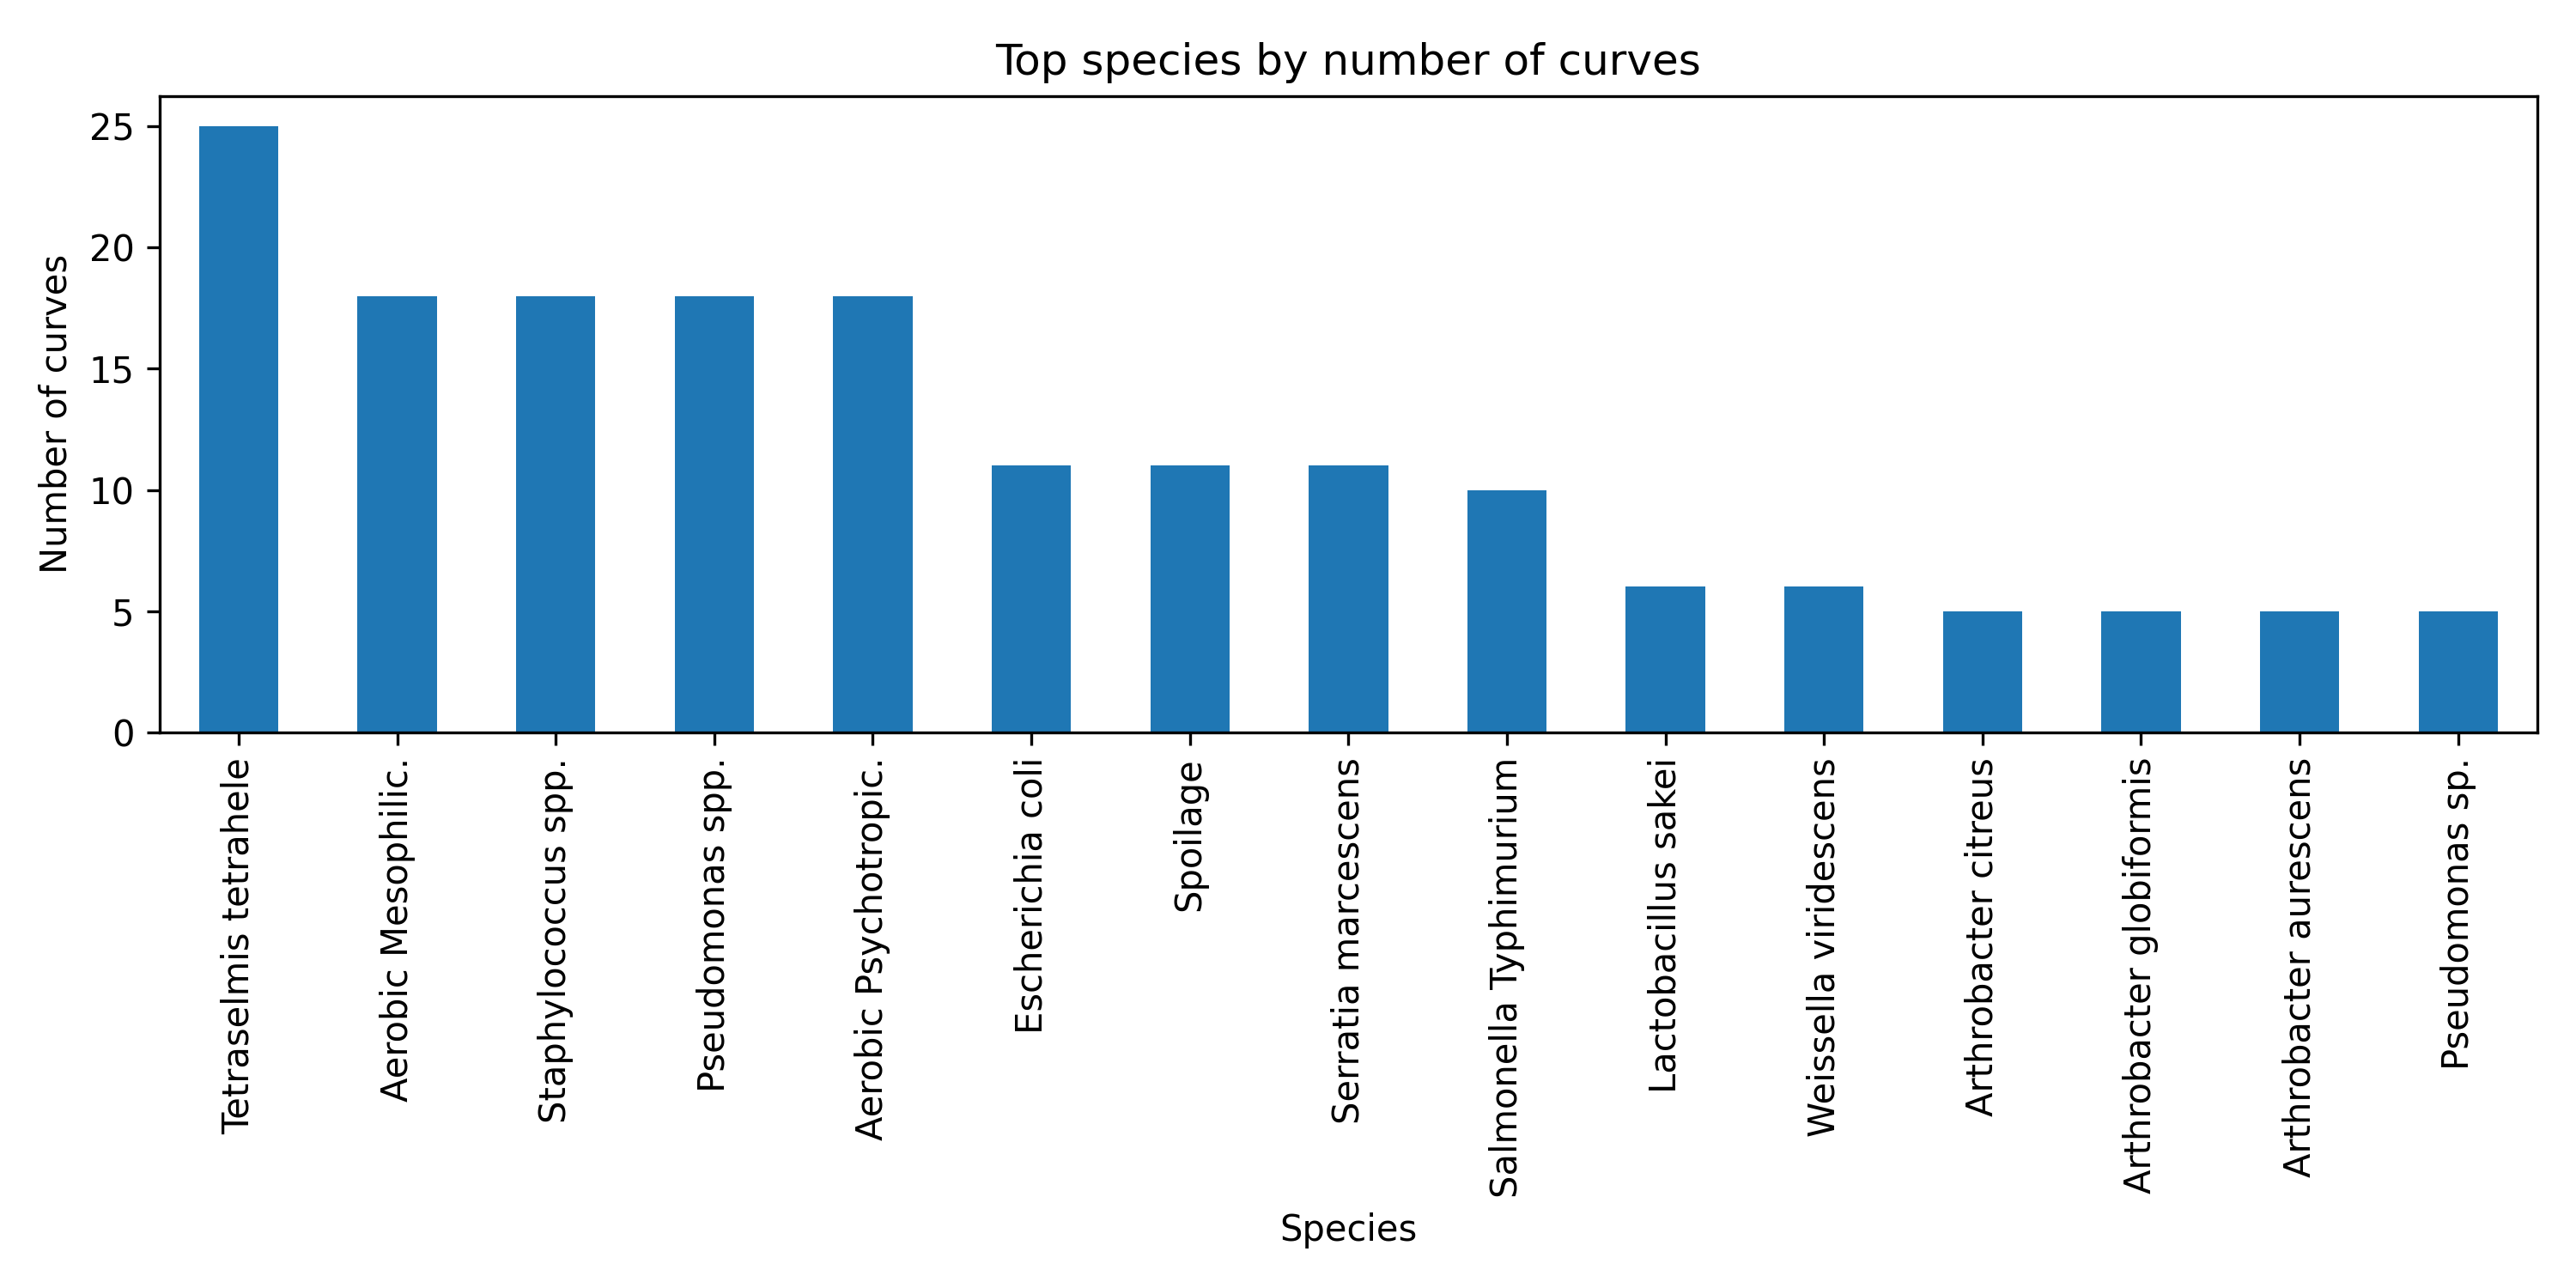
\includegraphics[width=0.95\textwidth]{species_curve_counts.png}
    \caption{Top species by number of growth curves in the cleaned dataset. The data were taxonomically broad, but several species contributed disproportionately large numbers of curves.}
    \label{fig:speciescounts}
\end{figure}

\subsection{Model fitting performance}

Both candidate models fitted the vast majority of curves successfully. Across 297 curves and two models per curve, this produced 594 fitting attempts. Gompertz fitting succeeded for all curves, while logistic fitting failed once, giving a success rate of 99.66\% for logistic and 100\% for Gompertz. The single logistic failure occurred because the optimiser exceeded the maximum number of function evaluations.

Representative fitted curves showed that both models often gave very similar predictions for monotonic sigmoidal trajectories (Figure~\ref{fig:repfits}). However, several curves displayed post-peak declines or highly irregular shapes, and in these cases both models fit the early growth phase better than the later decline. This indicates that the main limitation in such cases is not optimisation failure but model form.

\begin{figure}[p]
    \centering
    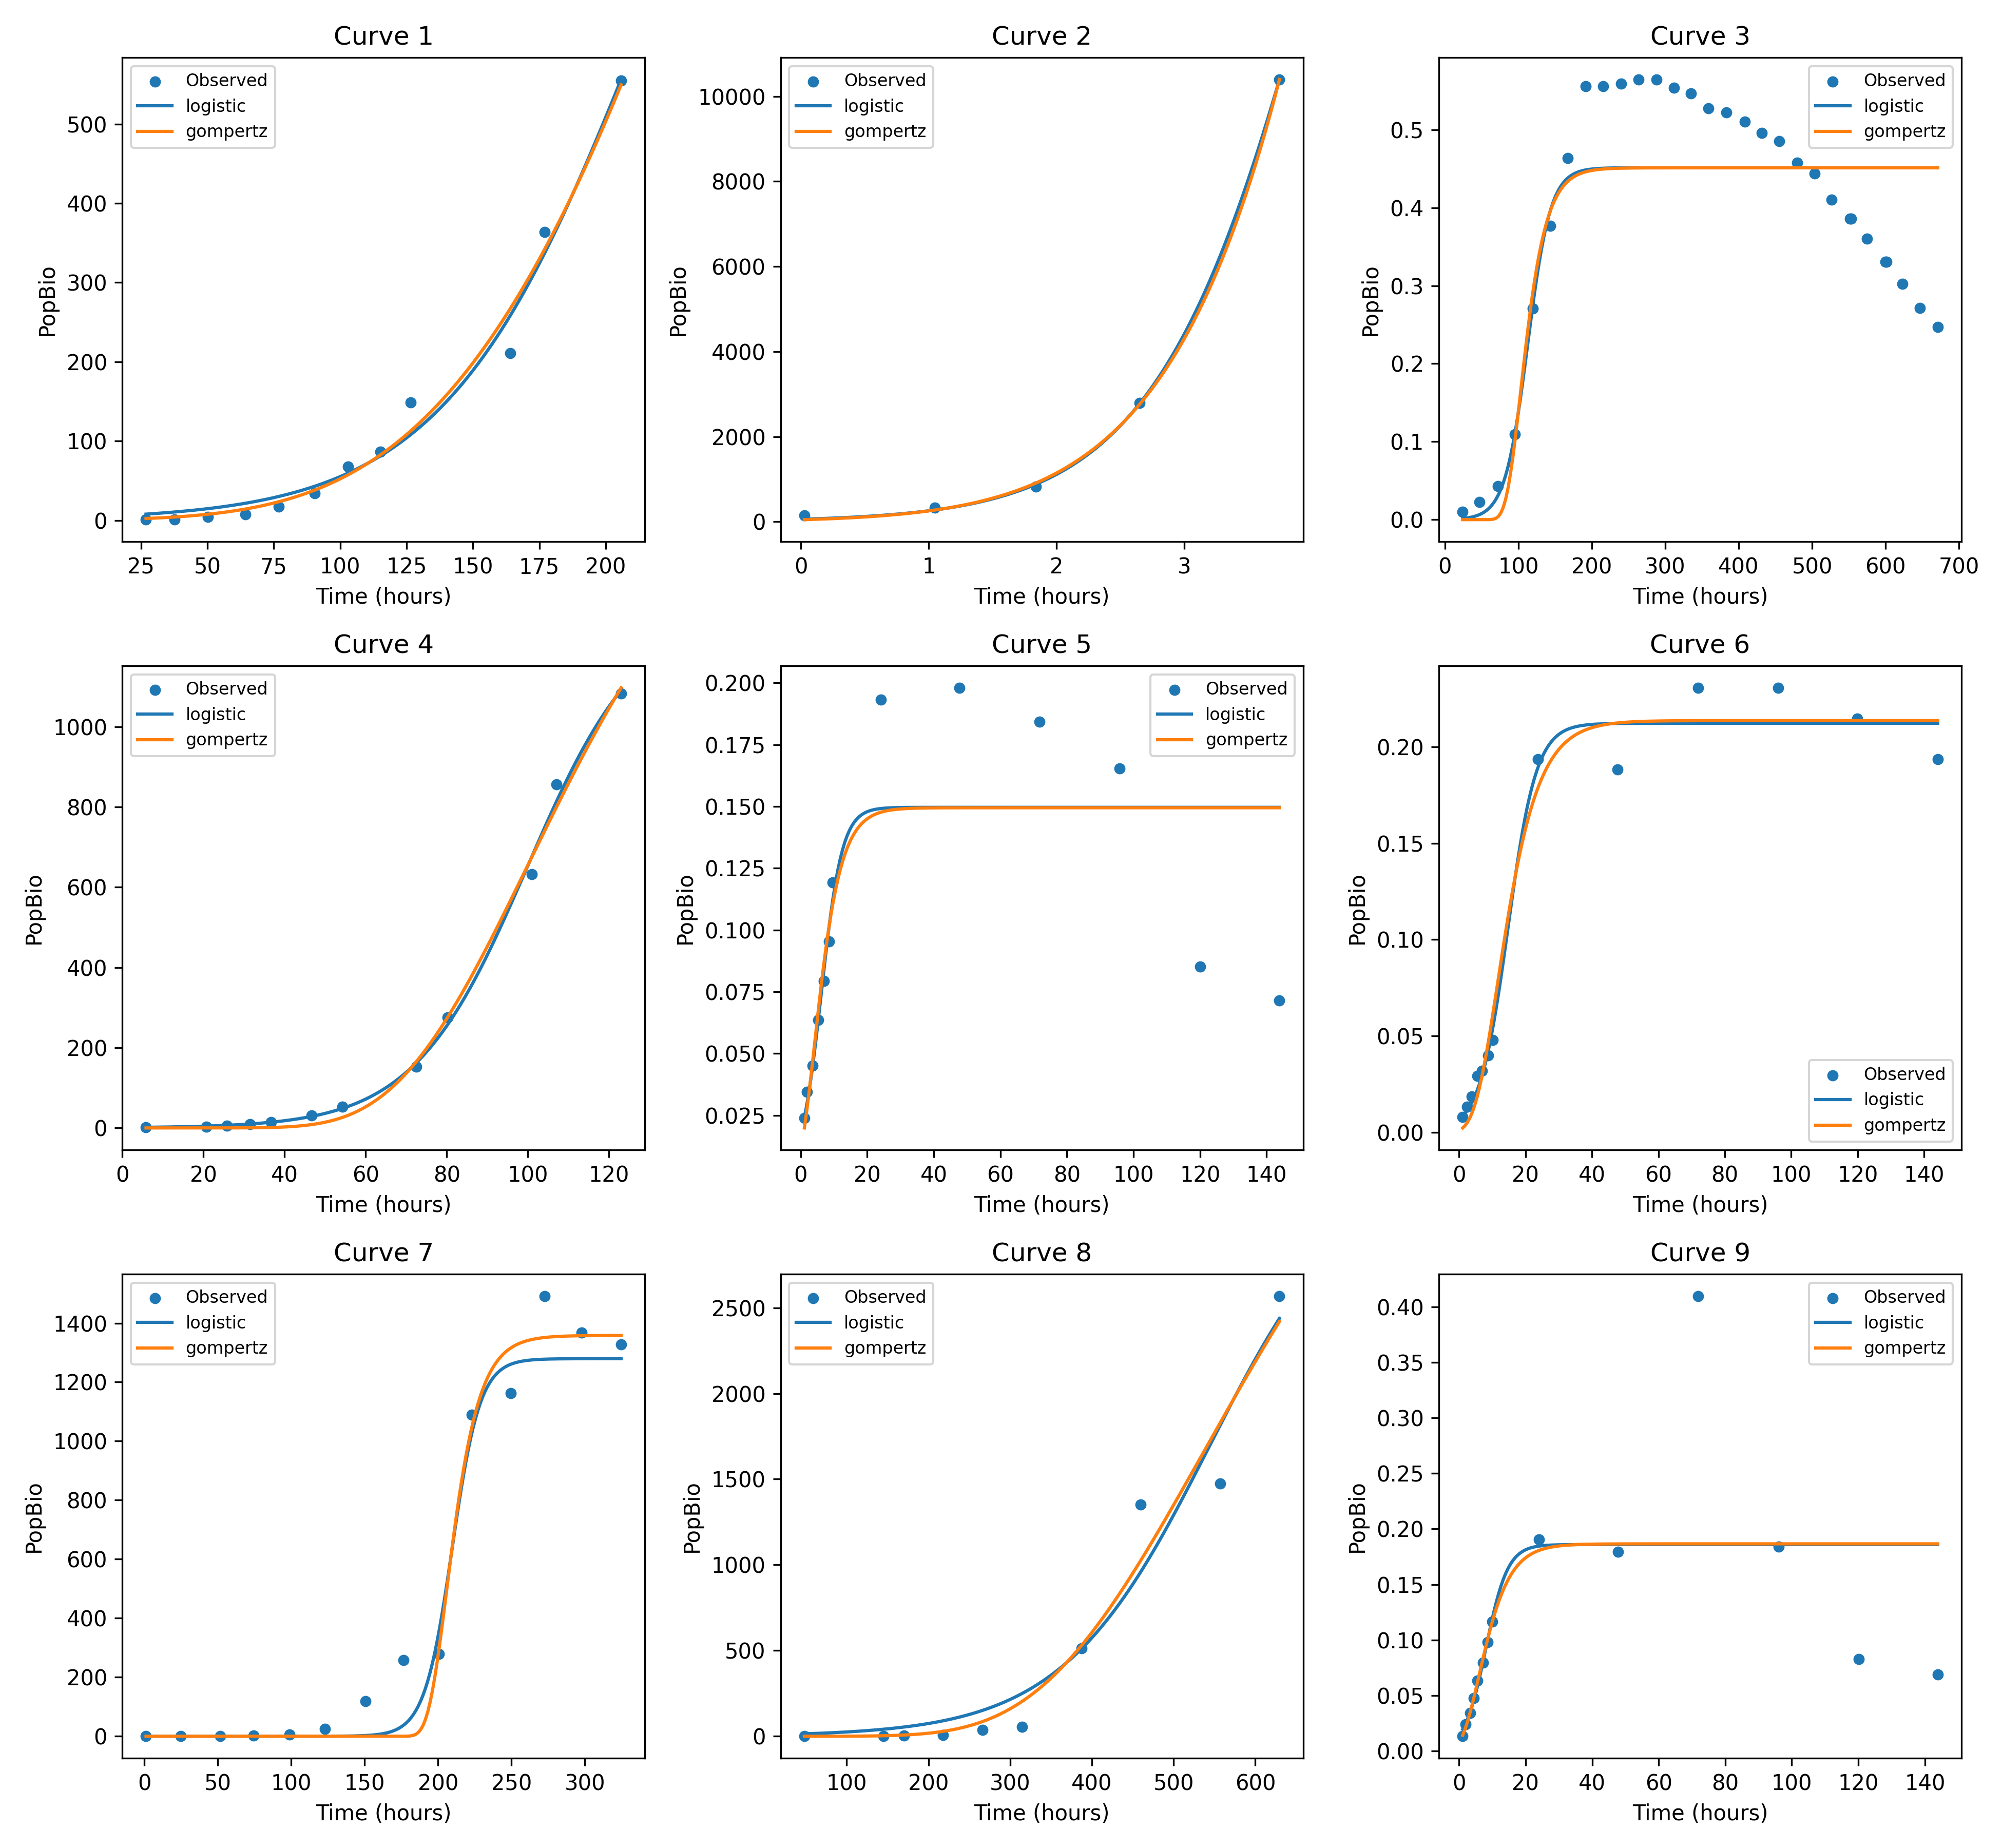
\includegraphics[width=\textwidth]{representative_curve_fits.png}
    \caption{Representative empirical growth curves and fitted logistic and Gompertz models. Both models generally captured monotonic sigmoidal growth well, but neither model described curves with strong post-peak decline particularly well.}
    \label{fig:repfits}
\end{figure}

\subsection{Model comparison}

Logistic models were selected as the best-fitting model for 176 of 297 curves, whereas Gompertz models were best for 121 curves (Figure~\ref{fig:bestcounts}). Thus, the logistic model provided the lower-AIC fit for the majority of curves in this dataset.

The distributions of AIC values for the two models were broadly similar, with substantial overlap and several extreme outliers for both models (Figure~\ref{fig:aicbox}). This overlap indicates that neither model dominated universally. Instead, model support varied among curves, even though the logistic model won more often overall.

Temperature-specific comparisons also suggested that model preference was context dependent (Figure~\ref{fig:besttemp}). Logistic remained the most common best-fitting model across many temperatures, but Gompertz was preferred more often at some temperature levels. Because sample size differed substantially among temperatures, these proportions should be interpreted cautiously where only a few curves were available.

\begin{figure}[H]
    \centering
    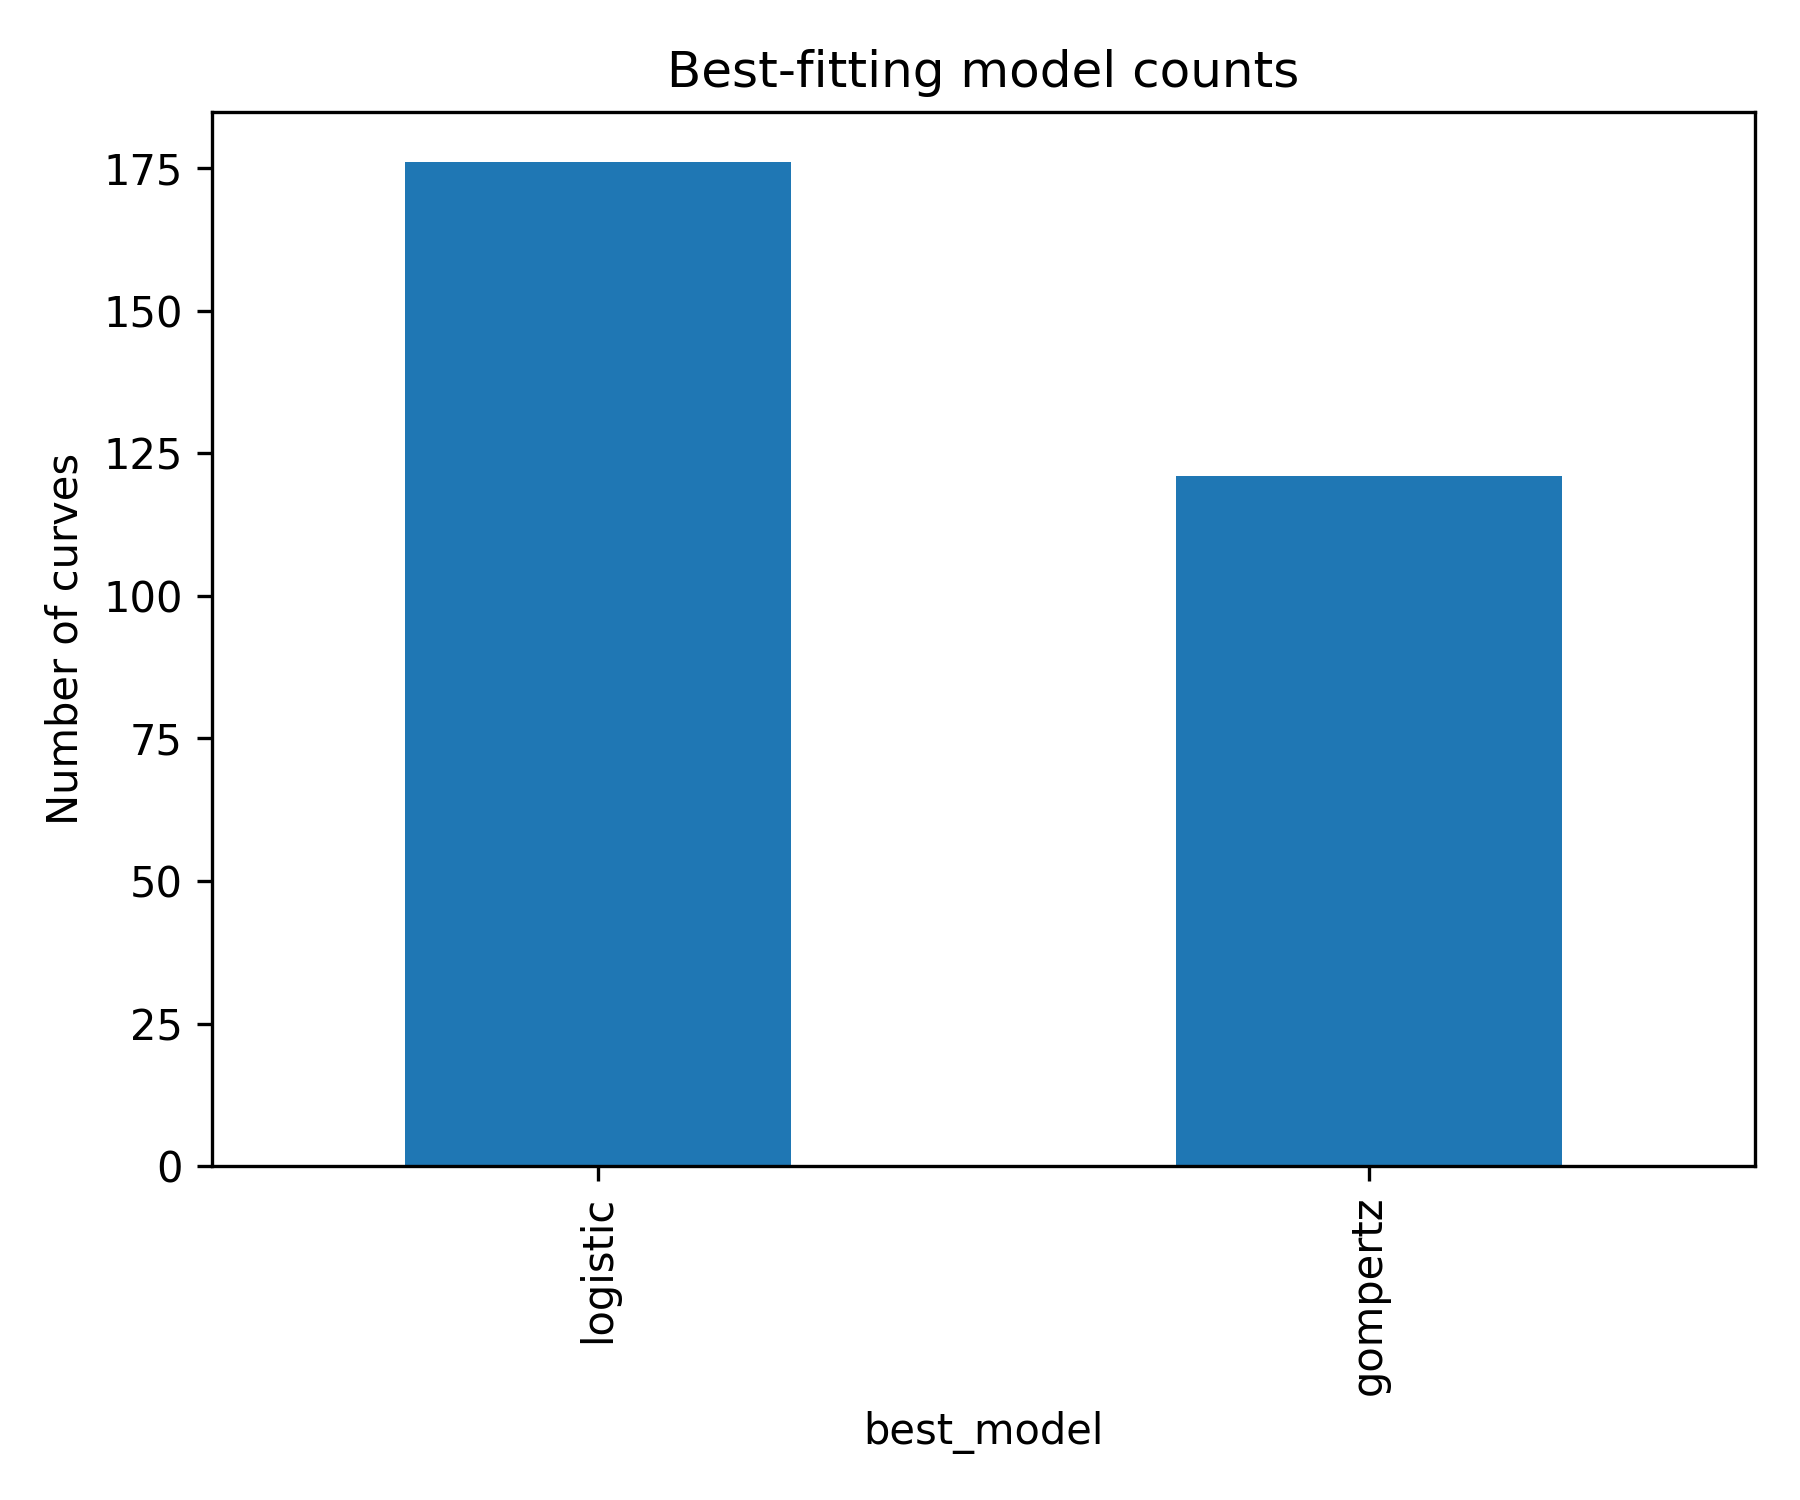
\includegraphics[width=0.65\textwidth]{best_model_counts.png}
    \caption{Number of curves for which each model had the lowest AIC. Logistic was selected more often overall than Gompertz.}
    \label{fig:bestcounts}
\end{figure}

\begin{figure}[H]
    \centering
    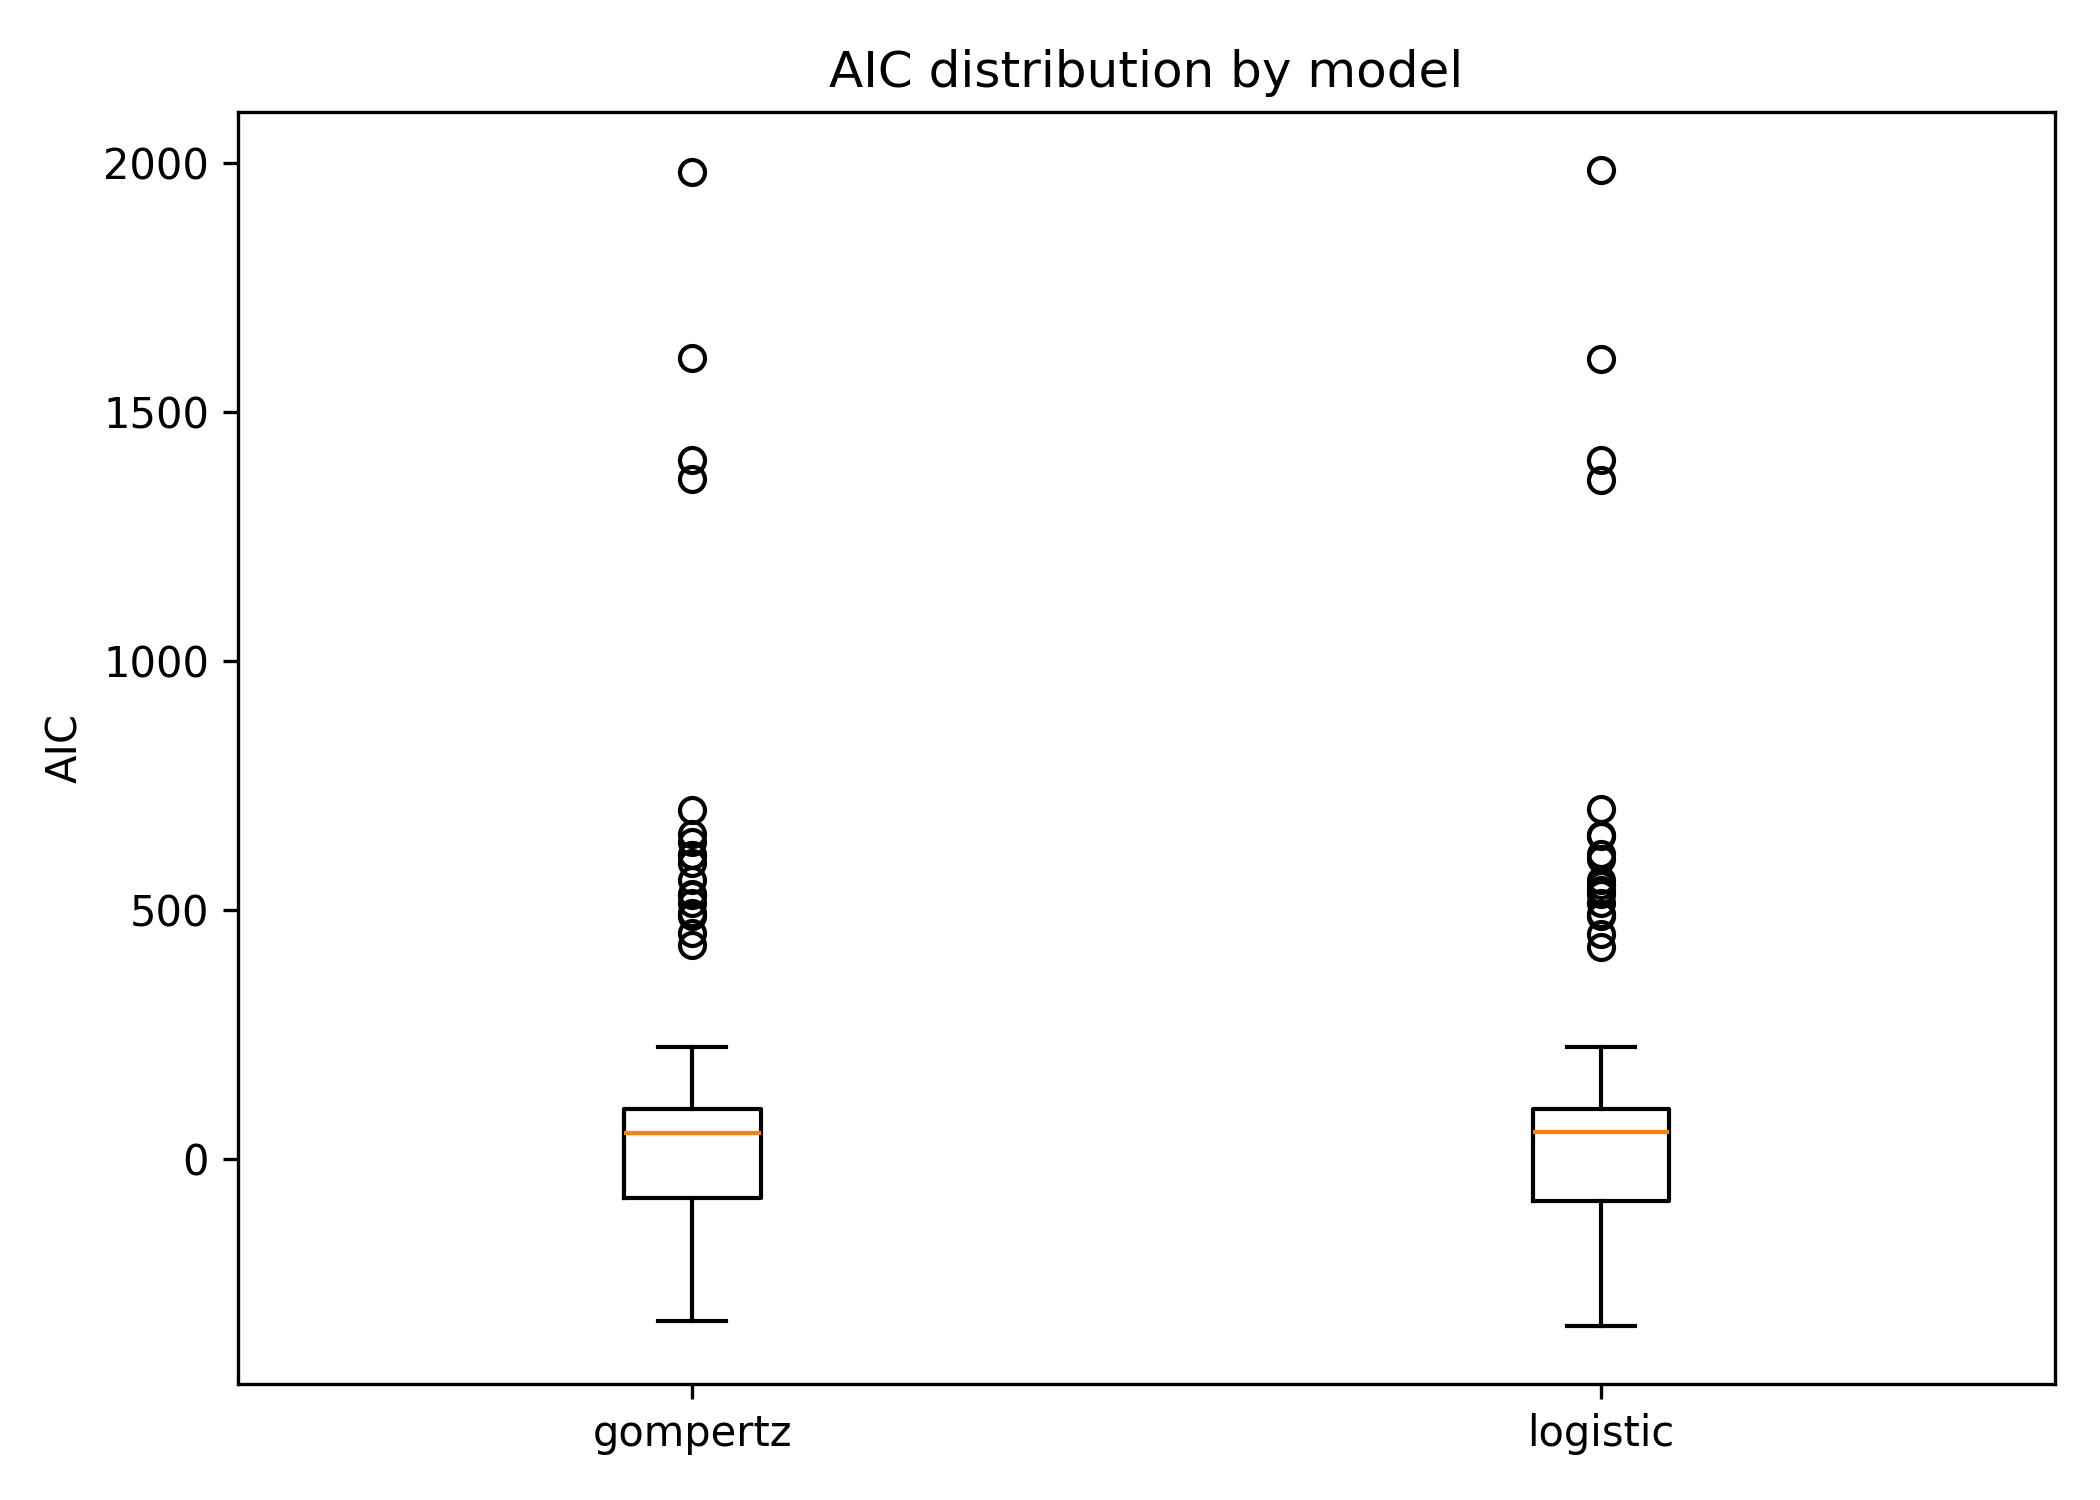
\includegraphics[width=0.75\textwidth]{aic_distribution_by_model.png}
    \caption{Distribution of AIC values across successful fits for each model. The two distributions overlapped strongly, but logistic achieved the lowest AIC more frequently overall.}
    \label{fig:aicbox}
\end{figure}

\begin{figure}[H]
    \centering
    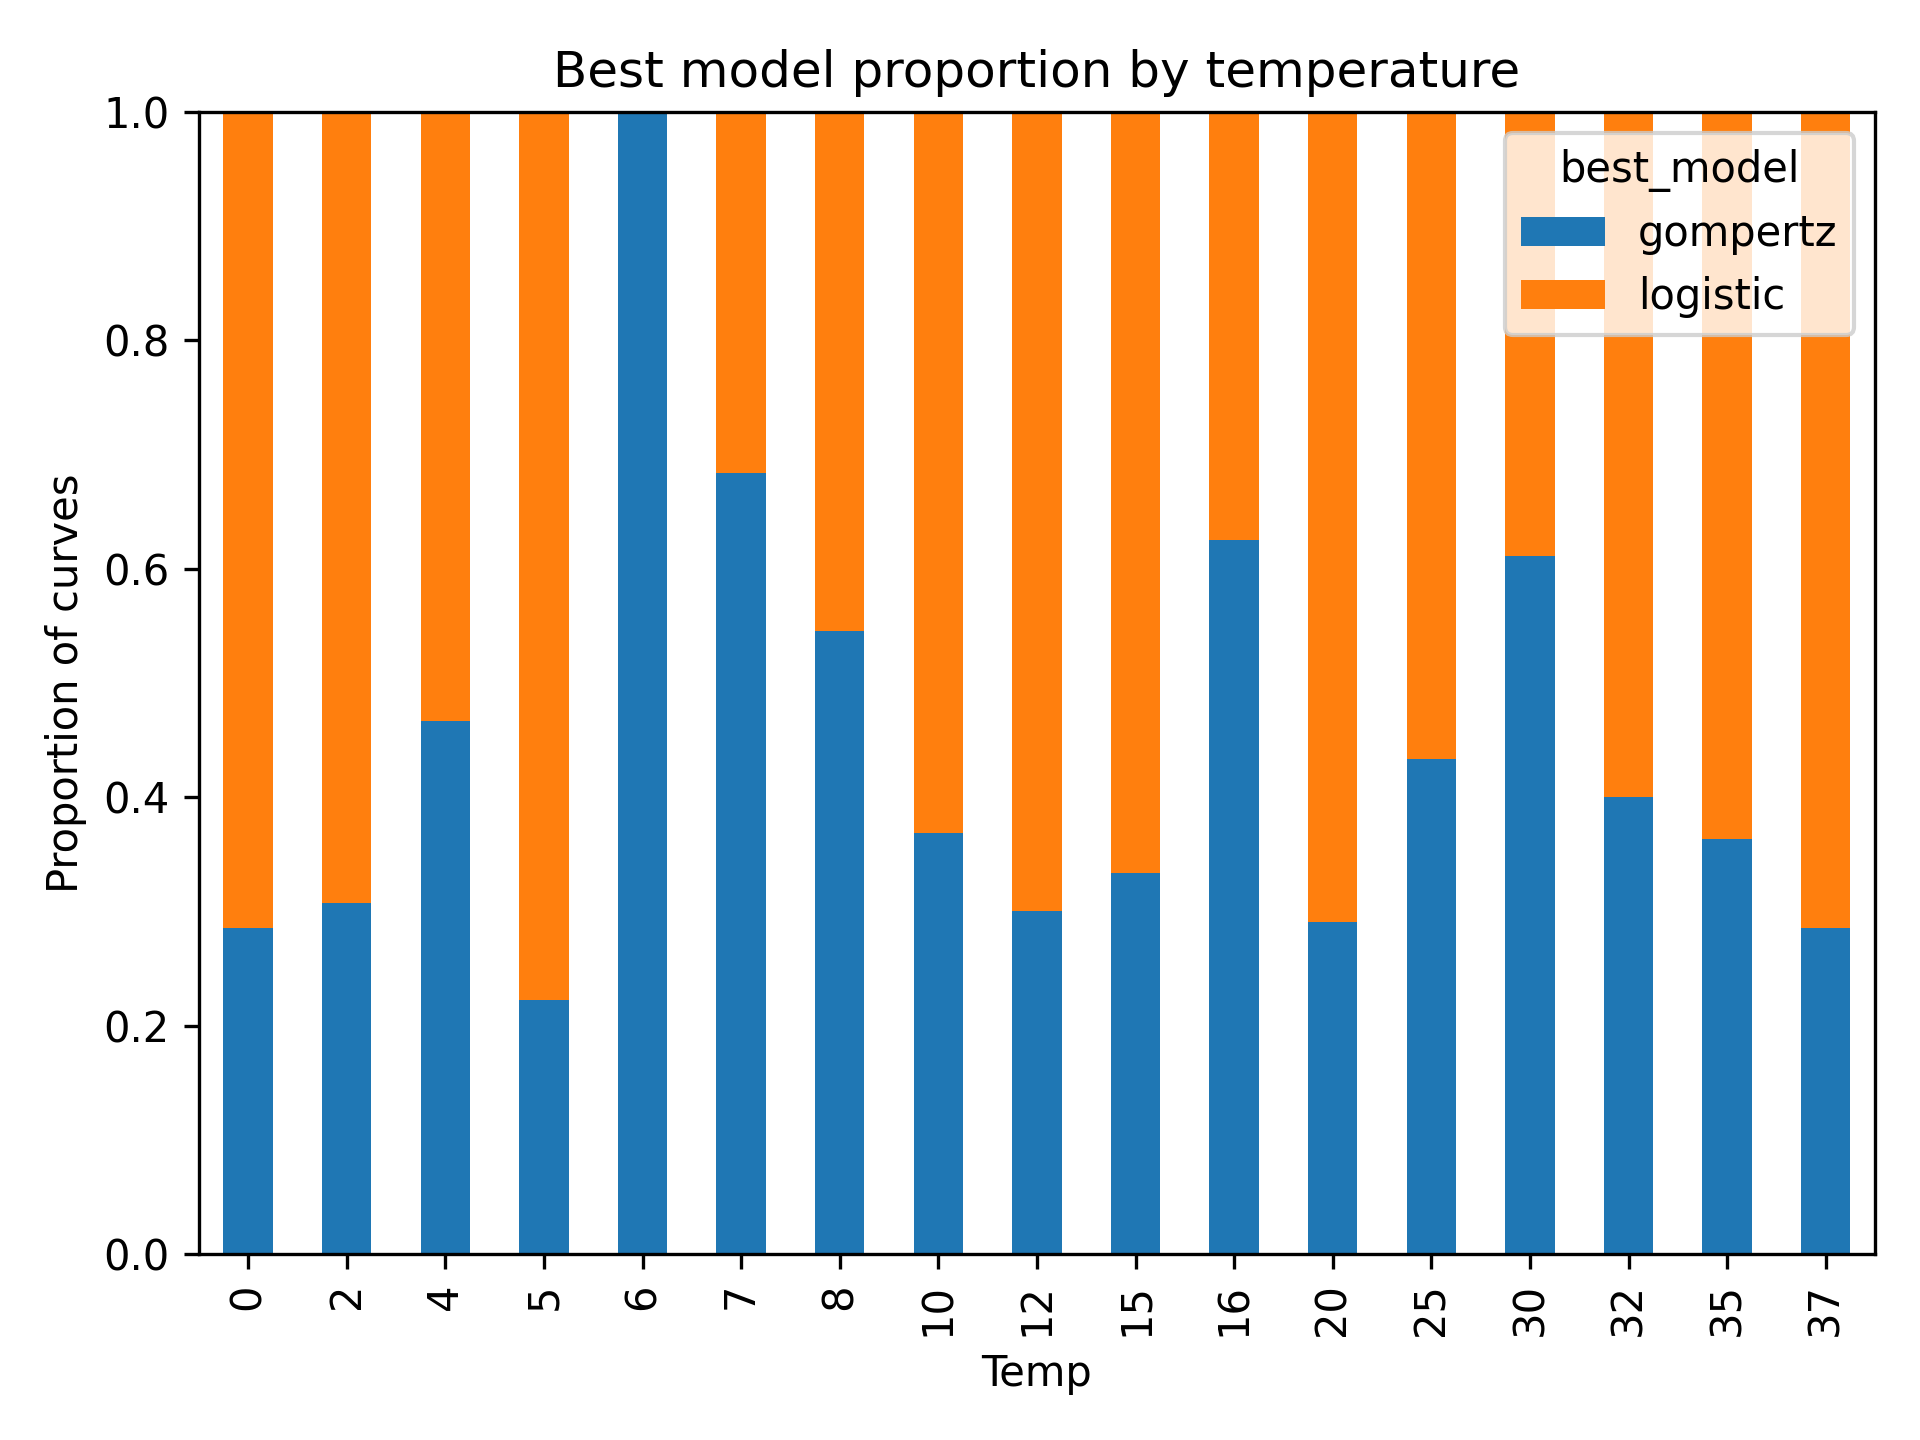
\includegraphics[width=0.85\textwidth]{best_model_by_temperature.png}
    \caption{Proportion of curves best described by each model at each temperature. Apparent temperature-specific shifts in model preference should be interpreted with caution because the number of curves per temperature varied widely.}
    \label{fig:besttemp}
\end{figure}

%========================
% Discussion
%========================
\section{Discussion}

Here I asked whether logistic or Gompertz growth models better described a diverse empirical dataset of microbial growth curves. Across 297 fitted curves, the logistic model was selected more often than the Gompertz model, although the difference was not overwhelming. This indicates that logistic growth provided the more robust general-purpose description of the dataset, while Gompertz remained a plausible alternative for many curves.

One likely reason for logistic's overall advantage is that many curves in the dataset were approximately monotonic and asymptotic, so a simple density-dependent form was sufficient to capture their shape. In these cases the added asymmetry of the Gompertz form did not necessarily provide enough improvement in residual error to compensate even under equal parameter count. At the same time, the fact that Gompertz was preferred for 121 curves shows that substantial heterogeneity existed across the dataset. Empirical microbial growth trajectories are not all equally symmetric, and some may contain lag phases or inflection structures that align better with a Gompertz-shaped trajectory \citep{Zwietering1990}.

The fitted examples also show an important limitation shared by both models. Several empirical curves increased and then declined after reaching a peak. Neither the logistic nor the Gompertz model can represent such decline, because both assume approach to an upper asymptote rather than overshoot followed by decrease. This means that some poor fits were not due to optimisation problems but to biological mismatch between candidate model and data. In other words, selecting the better of two models does not imply that either model is fully adequate for all observed dynamics.

This study also highlights the importance of careful model selection in ecology and microbiology. Comparing alternative models using information criteria is useful because it treats each model as a competing hypothesis about process and pattern \citep{JohnsonOmland2004}. Here, that comparison showed that logistic growth was more frequently supported, but not so strongly that Gompertz could be dismissed. The practical lesson is therefore not that one model should always be used, but that candidate models should be compared explicitly rather than chosen by convention.

There are several limitations to this analysis. First, the dataset combined curves measured in different biomass units, so parameter values were not directly comparable across all curves. I addressed this by performing model comparison within curves, but this still limits biological interpretation of global parameter distributions. Second, temperatures, taxa, and media were unevenly represented, which means that apparent context dependence in model support may partly reflect sampling imbalance. Third, only two sigmoidal models were considered. A broader candidate set, including models such as Baranyi or Richards forms, could better capture lag phases or other asymmetric shapes. Finally, one logistic fit failed to converge, and although this had negligible impact on the overall result, it is a reminder that non-linear fitting depends on both suitable starting values and model adequacy.

Overall, this project shows that logistic models more often outperform Gompertz models for this empirical microbial growth dataset, but that model choice remains context dependent. The strongest general conclusion is that simple sigmoidal models work well for many microbial growth curves, yet become inadequate when trajectories include decline or more complex phase structure. Future work should therefore compare a wider range of mechanistic and phenomenological growth models, especially for datasets that contain extended lag phases or post-peak decreases.

%========================
% References
%========================
\bibliography{references}

\end{document}